\documentclass[a4paper,twocolumn,11pt,nopdfoutputerror]{quantumarticle}
\usepackage[utf8]{inputenc}
\usepackage[T1]{fontenc}
\usepackage[english]{babel}
\usepackage{amsmath,amssymb,amsthm,mathtools}
\usepackage{braket}
\usepackage{graphicx}
\usepackage{booktabs}
\usepackage{siunitx}
\usepackage{microtype}
\usepackage{xcolor}
\usepackage[numbers,sort&compress]{natbib}
\usepackage[ruled,vlined]{algorithm2e}
\usepackage{enumitem}
\usepackage{multirow}
\usepackage{bbm}
\usepackage{makecell}

% ---------- macros ----------
\DeclareMathOperator{\Tr}{Tr}
\newcommand{\F}{\mathbb{F}}
\newcommand{\R}{\mathbb{R}}
\newcommand{\Pauli}{\mathcal{P}}
\newcommand{\synd}{\mathbf{s}}
\newcommand{\err}{\mathbf{e}}
\newcommand{\ehat}{\hat{\mathbf{e}}}
\newcommand{\llr}{\Lambda}
\newcommand{\Hmat}{\mathbf{H}}
\newcommand{\Gmat}{\mathbf{G}}
\newcommand{\Wmat}{\mathbf{W}}
\newcommand{\bvec}[1]{\mathbf{#1}}
\newcommand{\phat}{\hat{p}}
\newcommand{\concat}{\,\|\,}
\newcommand{\code}[3]{\ensuremath{[\![#1,#2,#3]\!]}}
\newcommand{\pending}[1]{\textcolor{red}{\textbf{[#1]}}}
\newtheorem{proposition}{Proposition}
\newtheorem{remark}{Remark}

\graphicspath{{./figures/}{./}}
\DeclareGraphicsExtensions{.pdf,.png,.jpg}

\usepackage{hyperref}
\hypersetup{colorlinks=true,citecolor=blue,linkcolor=blue,urlcolor=blue}

% ============================================================
%  TITLE
% ============================================================
\title{GNN-Augmented BP Architectures for QLDPC Decoding}

\author{Jothiradithya Sai Konduru}
\affiliation{Paradise Valley High School, Phoenix, AZ, USA}

\author{Anish Chedalla}
\affiliation{Paradise Valley High School, Phoenix, AZ, USA}

\author{Nithin Raveendran}
\affiliation{Department of Electrical and Computer Engineering,
             University of Arizona, Tucson, AZ, USA}
\email{nithin@arizona.edu}


\begin{document}
\maketitle

% ============================================================
%  ABSTRACT
% ============================================================
\begin{abstract}
Bivariate bicycle (BB) quantum low-density parity-check (QLDPC) codes
combine finite encoding rate with low-weight checks, but their loopy
Tanner graphs remain challenging for iterative decoding. We study a
Tanner-graph neural network (\textsc{TannerGNN}) that adds qubit-wise
log-likelihood corrections to belief propagation (BP) under biased CSS
noise. The network is trained with a per-qubit focal loss on the sampled
error, and its checkpoint is selected with 10-iteration flooding BP. On
the $\code{72}{12}{6}$ BB code at $p=0.04$ and $\eta=20$, it reduces the
logical error rate (LER) of that decoder by $12.5\%\pm0.6\%$ on 20{,}000
held-out syndromes (five training seeds; paired McNemar $p<10^{-36}$ for
every seed). The gain does not transfer to a stronger reference decoder,
serial min-sum BP-OSD: the correction never improves it and, after Holm
correction, is significantly worse for 11 of the 15 seed and
error-rate pairs with $p\geq0.03$. Most BP-OSD failures are also BP
failures, the GNN mainly repairs shots on which BP converges slowly and
which BP-OSD already decodes, and weight-three errors that cover half of a
stabilizer defeat BP with or without the GNN but never BP-OSD. Baseline
experiments show that BP schedule, update rule, iteration count and OSD
settings change the LER by orders of magnitude, and we prove that
uniformly rescaling the channel LLRs cannot change the hard decisions of
unclipped min-sum BP. Revealing the true per-qubit error rates, by
contrast, reduces the BP-OSD LER by up to 88\% under synthetic
heterogeneous noise and by 55\% under circuit-level noise.
\end{abstract}

% ============================================================
%  I. INTRODUCTION
% ============================================================
\section{Introduction}

Bivariate bicycle (BB) codes provide a concrete finite-length setting in
which QLDPC codes combine non-vanishing encoding rate, weight-six
stabilizer checks, and syndrome-extraction circuits compatible with
low-degree connectivity~\cite{Bravyi2024Memory}. IBM's current
fault-tolerant architecture is explicitly based on BB codes, making the
finite-length decoding behavior of this family practically relevant as
well as theoretically interesting~\cite{IBMRoadmap2025,Yoder2025TourDeGross}. The canonical
examples include the $\code{72}{12}{6}$, $\code{144}{12}{12}$, and
$\code{288}{12}{18}$ codes studied here.

The decoding bottleneck is not the absence of efficient iterative
algorithms, but their finite-length failure modes. BP is attractive
because its message updates are local and parallelizable, yet short
cycles and degeneracy in QLDPC Tanner graphs create correlated messages
and non-convergent or incorrect fixed points~\cite{Roffe2020Landscape}.
OSD post-processing can recover many BP failures, while recent learned
decoders use graph neural networks (GNNs) either to replace BP or to
intervene between BP stages~\cite{Gong2024GNN,Maan2025MLBP}. These
approaches make the choice of baseline unusually consequential: a neural
correction developed for one BP schedule or stopping rule need not
address the residual failures of a stronger decoder.

A second issue is adaptivity. Hardware noise is neither spatially nor
temporally uniform, and calibration information can therefore be useful
to a decoder. However, three distinct sources of information should not
be conflated: a global estimate of the physical error rate, spatially
resolved per-qubit calibration data, and syndrome history. A decoder may
respond differently to each. In particular, changing the magnitude of a
uniform channel prior has a restricted effect on min-sum BP, whereas
per-qubit priors can change the relative reliability ordering that drives
both BP and OSD.

We study a GNN-augmented BP pipeline with two questions in view:
\emph{what gain does the learned correction provide relative to the BP
decoder it is developed with, and what additional information is needed
for noise adaptation?} We compare decoder configurations, training and
evaluation baselines, and different forms of calibration information to
isolate the source of the observed performance changes.

\subsection{Related work}\label{sec:related}

Quantum Tanner graphs combine short cycles with degeneracy, and both
cause non-convergence and finite-length error floors in
BP~\cite{MacKay2004Sparse,Poulin2008Iterative,Roffe2020Landscape}.
Trapping-set analysis makes these failures structural rather than
mysterious: specific subgraphs, including symmetric configurations created
by stabilizers, can trap iterative decoders~\cite{Raveendran2021Trapping},
and degeneracy itself can be exploited inside BP~\cite{Kuo2022Degeneracy}.

Several families of methods repair such failures, with different latency
and complexity trade-offs. OSD post-processing~\cite{Fossorier1995OSD,Panteleev2021QLDPC,Roffe2020Landscape}
is the most widely used reference. Alternatives include stabilizer
inactivation~\cite{duCrest2022Inactivation},
check-agnosia~\cite{duCrest2024CheckAgnosia}, localized statistics
decoding~\cite{Hillmann2025LSD}, syndrome-based linear
programming~\cite{Javed2026LP}, collective bit
flipping~\cite{Chytas2025Collective}, and trapping-set-aware iterative
decoders of linear complexity~\cite{Pradhan2026Linear}. For BB codes in
particular, recent work targets real-time decoding: Relay-BP~\cite{Muller2025Relay},
graph rewiring with ensembles of normalized min-sum
decoders~\cite{Maan2026Correlated}, diversity and ensemble
methods~\cite{GarciaHerrero2026Diversity}, ambiguity
clustering~\cite{Wolanski2024Ambiguity}, and hardware implementations of
BP-OSD~\cite{Bascones2025FPGA}.

Learned decoders either modify BP messages or take over part of the
inference. Neural BP with a degeneracy-aware loss~\cite{Liu2019Neural},
GNN stages interleaved with BP~\cite{Gong2024GNN}, learned message
passing~\cite{Maan2025MLBP}, circuit-level neural decoders for BB
codes~\cite{Blue2026MLBB}, and calibration-conditioned
decoders~\cite{Stein2026FiLM} report both strong gains and limits in
scaling and transfer. In this landscape serial min-sum BP-OSD is a useful,
fully specified reference decoder, not the state of the art, and we use it
only in that role. Our question is narrower: what a learned LLR correction
gains relative to the BP configuration it is developed with, whether that
gain survives a stronger reference decoder, and what side information
adaptation actually needs.

\subsection{Contributions}\label{sec:contributions}

Our main findings are:
\begin{enumerate}[leftmargin=*,topsep=3pt,itemsep=3pt]
\item \textbf{A held-out GNN gain over the BP decoder it is developed
with.} On $\code{72}{12}{6}$ at $p=0.04$ and $\eta=20$,
\textsc{TannerGNN}+flooding BP reduces LER by $12.5\%\pm0.6\%$ on
20{,}000 held-out syndromes over five training seeds (McNemar
$p<10^{-36}$ for every seed). The training rates span
$p\in[0.005,0.045]$; at $p=0.06$, outside that range, the reduction is
$10.6\%\pm0.7\%$. The whole gain is in the $Z$ component; adding the
correction to the $X$ component as well only adds failures there
(Sec.~\ref{sec:gnn_positive}).

\item \textbf{Baseline configuration and alignment can dominate the
apparent learned gain.} Serial min-sum BP with OSD post-processing is
substantially stronger than the flooding BP used to select the GNN
checkpoint. The same learned correction never improves this stronger
decoder and, after Holm correction, is significantly worse for 11 of
the 15 seed and error-rate pairs with $p\geq0.03$. A paired failure-set
analysis shows that 93\% of BP-OSD failures are also BP failures
(61\% the other way) and that most shots the GNN repairs are
already decoded by BP-OSD. Separate experiments on
$\code{288}{12}{18}$ show order-of-magnitude sensitivity to BP schedule,
update rule, iteration count, and OSD settings. The decoder used for
model selection and the evaluation decoder are therefore part of the
experimental condition rather than interchangeable implementations of
``BP''
(Secs.~\ref{sec:baseline} and~\ref{sec:mismatch}).

\item \textbf{A recurring BP failure that the GNN does not repair.} When
a weight-three $Z$ error covers half of a weight-six stabilizer, the error
and its stabilizer complement are equally likely and logically
equivalent. BP, 100-iteration BP and GNN-BP fail on every such shot in our
test sets and BP-OSD on none; the GNN's bitwise loss gives both halves the
same target, so it cannot learn to break the tie
(Secs.~\ref{sec:training} and~\ref{sec:mismatch}).

\item \textbf{Global prior scaling and spatial calibration carry
different information.} We prove that hard decisions of unclipped
min-sum BP are invariant to a uniform positive rescaling of the channel
LLRs within a CSS component. This result limits adaptivity obtained only
by changing a uniform BP prior; it does not rule out a learned network
using a global noise scalar as context. In synthetic heterogeneous-noise
experiments, providing the true per-qubit rates to BP-OSD yields large
oracle improvements, motivating spatially resolved calibration inputs.
Because code size and operating point co-vary in these experiments, we do
not attribute the cross-code trend to distance alone
(Secs.~\ref{sec:invariance} and~\ref{sec:oraclegap}).
\end{enumerate}
\section{Background}\label{sec:background}

\subsection{CSS codes and bivariate bicycle construction}

A CSS code~\cite{Calderbank1996Good,Steane1996Error} is defined by
matrices $\Hmat_x, \Hmat_z \in \F_2^{m \times n}$ with
$\Hmat_x \Hmat_z^\top = \mathbf{0}$. The syndrome of an error
$(e_x, e_z)$ decomposes as
$s_x = \Hmat_x e_z$,
$s_z = \Hmat_z e_x$
over $\F_2$, so $X$- and $Z$-type errors are decoded independently.
This CSS independence is structurally important for the results
of Sec.~\ref{sec:invariance}.

Bivariate bicycle codes~\cite{Bravyi2024Memory} are constructed
over the group algebra $\F_2[x,y]/(x^\ell-1,\,y^m-1)$. Polynomials
$A(x,y)$ and $B(x,y)$ yield circulant block matrices:
\begin{equation}
\Hmat_x = [\mathbf{A} \mid \mathbf{B}], \qquad
\Hmat_z = [\mathbf{B}^\top \mid \mathbf{A}^\top].
\label{eq:bb}
\end{equation}
We study three codes (Table~\ref{tab:codes}).

\begin{table*}[t]
\centering
\caption{Bivariate bicycle codes studied in this work, with
         generator polynomials from \cite{Bravyi2024Memory};
         $\Hmat_x$ and $\Hmat_z$ follow Eq.~\eqref{eq:bb} over
         $\F_2[x,y]/(x^\ell-1,\,y^m-1)$. The names ``gross'' and
         ``two-gross'' follow IBM's usage~\cite{Yoder2025TourDeGross}.}
\label{tab:codes}
\begin{tabular}{@{}llcccccccc@{}}
\toprule
Code & Name & $n$ & $k$ & $d$ & Rate & $\ell$ & $m$ & $A(x,y)$ & $B(x,y)$ \\
\midrule
$\code{72}{12}{6}$   & ---       &  72 & 12 &  6 & 1/6  &  6 &  6 & $x^3+y+y^2$   & $y^3+x+x^2$ \\
$\code{144}{12}{12}$ & gross     & 144 & 12 & 12 & 1/12 & 12 &  6 & $x^3+y+y^2$   & $y^3+x+x^2$ \\
$\code{288}{12}{18}$ & two-gross & 288 & 12 & 18 & 1/24 & 12 & 12 & $x^3+y^2+y^7$ & $y^3+x+x^2$ \\
\bottomrule
\end{tabular}
\end{table*}

\subsection{Belief propagation and its failure modes}\label{sec:bp}

Min-sum BP on a CSS Tanner graph iterates variable-to-check and
check-to-variable messages for $T$ steps. For a check $c_j$ with measured
syndrome bit $s_j$ and a neighboring variable $v_i$,
\begin{align}
\mu_{v_i \to c_j}^{(t)}
&= \llr_i + \!\!\sum_{j' \in \mathcal{N}(i)\setminus j}\!\!
\mu_{c_{j'} \to v_i}^{(t-1)},
\label{eq:vtc}\\
\mu_{c_j \to v_i}^{(t)}
&= (-1)^{s_j}
\!\!\prod_{i' \in \mathcal{N}(j)\setminus i}\!\!
\mathrm{sgn}\!\left(\mu_{v_{i'}\to c_j}^{(t)}\right) \notag\\
&\quad \times
\!\!\min_{i'\in\mathcal{N}(j)\setminus i}\!\!
\left|\mu_{v_{i'}\to c_j}^{(t)}\right|.
\label{eq:ctv}
\end{align}
CSS decoding separates the $X$ and $Z$ components, processing each with
its respective parity-check matrix. Under the noise model of
Sec.~\ref{sec:noise} the matched channel LLRs are
$\llr_{z,i} = \ln\bigl((1-p_z)/p_z\bigr)$ for $Z$ errors and
$\llr_{x,i} = \ln\bigl((1-p_x)/p_x\bigr)$ for $X$ errors; at $p=0.04$ and
$\eta=20$, $p_z=0.0381$, $p_x=0.0019$ and
$\llr_{x}/\llr_{z}=6.26/3.23\approx1.94$. Each experiment below states
which prior every decoder receives.

The Tanner graphs of the finite-length BB codes considered here contain
many short cycles. Message reuse around these cycles creates statistical
dependencies that are absent on a tree and can lead BP to oscillate,
converge to a syndrome-inconsistent estimate, or converge to the wrong
logical class. We therefore treat short-cycle structure as a finite-length
decoder mechanism to be measured, rather than attributing every cycle
directly to the CSS orthogonality condition. Post-processing methods
including ordered-statistics decoding (OSD)~\cite{Fossorier1995OSD}
recover many such failures but add $O(n^3)$ worst-case complexity.
As shown in Sec.~\ref{sec:baseline}, the specific OSD
\emph{configuration}---schedule, base method, and iteration count---can
change LER by more than two orders of magnitude on the same code. We
therefore report these settings explicitly in the comparisons below.

\subsection{Noise models}\label{sec:noise}

We use a $Z$-biased CSS component-noise model with $\eta = 20$:
\begin{equation}
p_z = \frac{p\eta}{\eta+1}, \qquad p_x = \frac{p}{\eta+1}.
\label{eq:bias}
\end{equation}
Each data qubit independently suffers a $Z$ flip with probability $p_z$
and an $X$ flip with probability $p_x$. No separate $Y$ channel is
sampled: a qubit carries a $Y$ error only if it receives both flips,
which happens with probability $p_xp_z\approx p^2/22$, so this is not
depolarizing noise. Syndromes are $s_x=\Hmat_x e_z$ and
$s_z=\Hmat_z e_x$, and the two components are decoded separately.
Two kinds of temporal variation appear, both motivated by fluctuating
two-level systems~\cite{Klimov2018,Carroll2022}: the GNN training data
modulate the global rate sinusoidally, $p(t) = p_0 + A\sin(2\pi t/T)$
(Sec.~\ref{sec:training}), and the drift experiment of
Sec.~\ref{sec:drift} lets the rate of each qubit follow its own
Ornstein--Uhlenbeck process. Which noise parameters a decoder sees is
stated with each experiment.

% ============================================================
%  III. THE ADAPTIVEBP FRAMEWORK
% ============================================================
\section{The \textsc{AdaptiveBP} Framework}\label{sec:methods}

This section describes the model evaluated in Sec.~\ref{sec:results}. Two
further variants, FiLM conditioning and an interleaved GNN-BP pipeline,
are described in Appendix~\ref{app:variants}; they are not evaluated.

\subsection{\textsc{TannerGNN}}\label{sec:tannergnn}

\textsc{TannerGNN} operates on the unified CSS Tanner graph, with
edges distinguished by type $\tau \in \{X\text{-check},Z\text{-check}\}$.
Each node receives a 4-dimensional feature vector whose first entry is
a value and whose last three entries one-hot encode the node type: a
variable node $v_i$ receives $\bvec{x}_i=[\ell,1,0,0]$, and an $X$-check
($Z$-check) node $c_j$ receives $[s_j,0,1,0]$ ($[s_j,0,0,1]$), where
$s_j$ is its syndrome bit. The prior LLR $\ell=\ln\bigl((1-p)/p\bigr)$ is
computed from the total physical error rate $p$ of the shot, not from
$p_z$ or $p_x$: for the drifting training streams it is the
instantaneous rate $p(t)$, and for the test sets the fixed $p$. The same
$\ell$ is the channel prior of both CSS components in the flooding-BP
decoders of Sec.~\ref{sec:results}. Its magnitude does not change
min-sum decisions (Sec.~\ref{sec:invariance}), but it sets the scale
against which the correction $\Delta_i$ acts.

An input projection maps features to hidden dimension $d_h$ ($d_h=32$
for the model of Sec.~\ref{sec:gnn_positive}) via
$\bvec{h}_i^{(0)} = \mathrm{ReLU}(\mathrm{LayerNorm}(\Wmat_\mathrm{proj}\bvec{x}_i))$.
Each of $L = 3$ message-passing layers applies separate edge-type
MLPs, optional attention weighting, and a GRU node update:
\begin{align}
\bvec{m}_i^{(\ell)} &= \sum_{j\in\mathcal{N}(i)}
  \mathrm{MLP}_{e,\tau(i,j)}^{(\ell)}\!\bigl(\bigl[\bvec{h}_i^{(\ell)},\bvec{h}_j^{(\ell)}\bigr]\bigr),
  \label{eq:msg}\\
\bvec{h}_i^{(\ell+1)} &= \mathrm{GRU}\!\bigl(\bvec{h}_i^{(\ell)},\;
  \bvec{m}_i^{(\ell)}\bigr).
  \label{eq:gru}
\end{align}
A readout MLP maps each variable node's final hidden state to a
per-qubit LLR correction: $\Delta_i = \mathrm{MLP}_\mathrm{read}(\bvec{h}_i^{(L)})$.

\begin{figure*}[t]
\centering
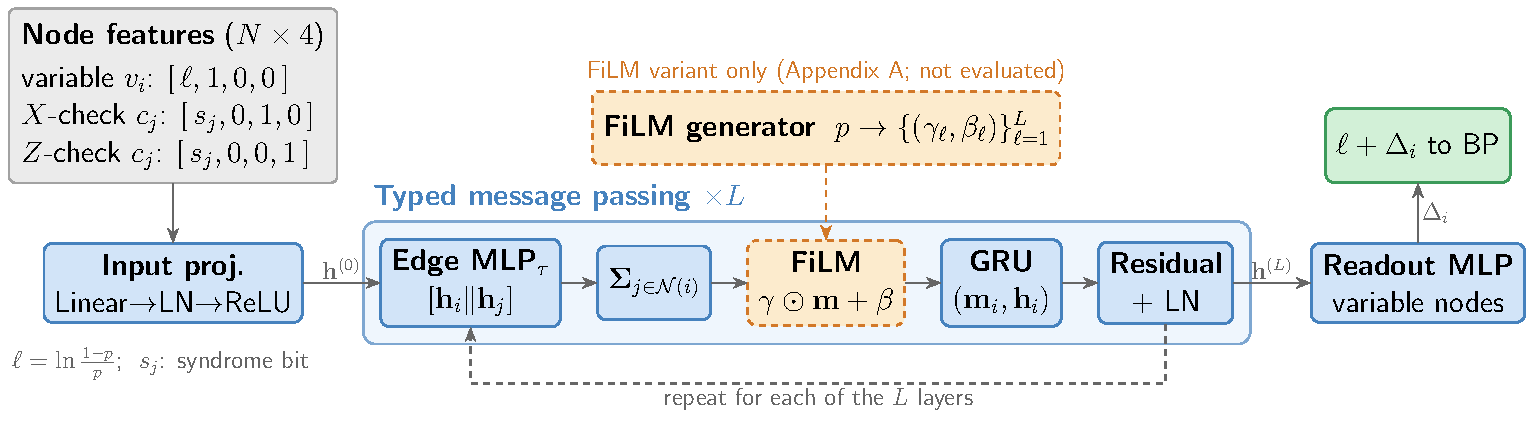
\includegraphics[width=\textwidth]{fig_tannergnn_arch}
\caption{\textsc{TannerGNN} architecture. Variable and check nodes
         exchange typed messages over $L=3$ layers via edge-type-specific
         MLPs; a GRU update with a residual connection and layer
         normalisation follows at each node, and a readout MLP on the
         variable nodes gives the LLR corrections. In the FiLM variant
         (dashed; Appendix~\ref{app:variants}), FiLM modulation scales the
         aggregated messages at each layer; the model of
         Sec.~\ref{sec:gnn_positive} does not use FiLM.}
\label{fig:tannergnn_arch}
\end{figure*}



\subsection{Training}\label{sec:training}

\begin{table}[t]
\centering
\footnotesize
\caption{Architecture and training configuration of the
         \textsc{TannerGNN} model of Secs.~\ref{sec:gnn_positive}
         and~\ref{sec:mismatch}.}
\label{tab:hparams}
\setlength{\tabcolsep}{3pt}
\begin{tabular}{@{}ll@{}}
\toprule
\multicolumn{2}{@{}l}{\textit{GNN architecture}} \\
\midrule
Layers $L$ / width $d_h$       & 3 / 32 \\
Edge types                      & 2 ($\Hmat_x$, $\Hmat_z$) \\
Node update                     & GRU, residual, layer norm \\
Node feature dim.               & 4 \\
FiLM / attention                & not used \\
Parameters                      & 39{,}329 \\
\midrule
\multicolumn{2}{@{}l}{\textit{Training}} \\
\midrule
Data                            & \makecell[l]{8{,}000 shots, sinusoidal drift,\\$p\in[0.005,0.045]$} \\
Prior feature $\ell$            & \makecell[l]{$\ln((1-p)/p)$, true $p$ of the shot,\\both components} \\
Loss                            & \makecell[l]{focal, $(\alpha,\gamma)=(0.25,2.0)$, on\\$q_j=\sigma(-(\ell+\Delta_j))$ vs.\ $e_z$;\\no syndrome term} \\
Optimizer                       & \makecell[l]{AdamW, lr $2\times10^{-3}$,\\weight decay $10^{-4}$} \\
Batch size / epochs             & 64 / 20, gradient clipping 1.0 \\
Checkpoint                      & \makecell[l]{fewest failures on\\4{,}000 validation shots} \\
Training seeds                  & 5 \\
BP for model selection          & \makecell[l]{flooding min-sum, scaling 0.8,\\10 iter.; not in the loss} \\
\midrule
\multicolumn{2}{@{}l}{\textit{Reference BP-OSD baseline}} \\
\midrule
Implementation                  & \texttt{ldpc} 2.4.1 \texttt{BpOsdDecoder} \\
\texttt{bp\_method}             & \texttt{ms} (min-sum) \\
\texttt{ms\_scaling\_factor}    & $0.8$ \\
\texttt{schedule}               & \texttt{serial} (layered) \\
\texttt{max\_iter}              & 100 \\
OSD (where used)                & \texttt{osd\_cs}, order 10 \\
\bottomrule
\end{tabular}
\end{table}

The model is trained as a per-qubit classifier of the sampled $Z$ error;
BP is not part of its loss. For a shot with prior LLR $\ell$ on every
qubit, the GNN outputs a correction $\Delta_j$ for each qubit $j$, giving
the corrected error probability $q_j=\sigma\bigl(-(\ell+\Delta_j)\bigr)$,
and the loss is the focal loss~\cite{Lin2017Focal} against the true $Z$
error $e_z$,
\begin{equation}
\mathcal{L}=-\frac{1}{Bn}\sum_{b=1}^{B}\sum_{j=1}^{n}
\alpha_{t}\,(1-q_{t})^{\gamma}\log q_{t},
\label{eq:loss}
\end{equation}
where $q_t=q_j$ and $\alpha_t=\alpha$ if $e_{z,j}=1$, and $q_t=1-q_j$
and $\alpha_t=1-\alpha$ otherwise, with $\alpha=0.25$ and $\gamma=2$; no
syndrome-consistency term is used. The computation graph is therefore
$(\ell,\synd)\to\textsc{TannerGNN}\to\Delta\to q\to\mathcal{L}$, and
gradients reach the GNN without passing through BP. Ten-iteration flooding
BP enters training only through model selection: after each of the 20
epochs the corrected priors $\ell+\Delta$ are decoded with that BP on
4{,}000 validation shots, and the epoch with the fewest failures is kept.
The training data are 8{,}000 shots from two sinusoidally drifting
streams, $p(t)=p_0+0.015\sin(2\pi t/500)$ with $p_0\in\{0.02,0.03\}$, so
the training rates span $p\in[0.005,0.045]$. Table~\ref{tab:hparams}
summarises the configuration.

The target is the sampled error $e_z$, so the loss is not
degeneracy-aware: an estimate that differs from $e_z$ by a stabilizer is
logically correct but is penalized like any other error. The extreme case
is an error that covers exactly half of a weight-six stabilizer $g$. Then
$e_z$ and $e_z\oplus g$ have the same weight and the same syndrome, so
they are equally likely and the network receives the same input for
both; the loss rewards treating the six qubits alike and gives no
incentive to prefer either half. Section~\ref{sec:mismatch} shows that
such configurations are a major cause of BP failures. Degeneracy-aware
objectives, such as that of Liu and Poulin~\cite{Liu2019Neural}, avoid
this problem; we did not use one.

\begin{remark}[One correction for two CSS components]
The GNN outputs one correction $\Delta_i$ per qubit and is trained on $Z$
errors only. In the experiments of
Sec.~\ref{sec:results} the same $\Delta_i$ is added to the prior $\ell$ of
both components, although the two error types differ: $X$ errors are
$\eta=20$ times rarer, and the matched LLRs differ by a factor
$\llr_x/\llr_z\approx1.94$ at $p=0.04$. Section~\ref{sec:gnn_positive}
measures the consequence and shows that adding $\Delta_i$ to the $Z$
component only is better.
\end{remark}

% ============================================================
%  IV. EXPERIMENTAL SETUP
% ============================================================
\section{Experimental Setup}\label{sec:setup}

\begin{figure*}[t]
\centering
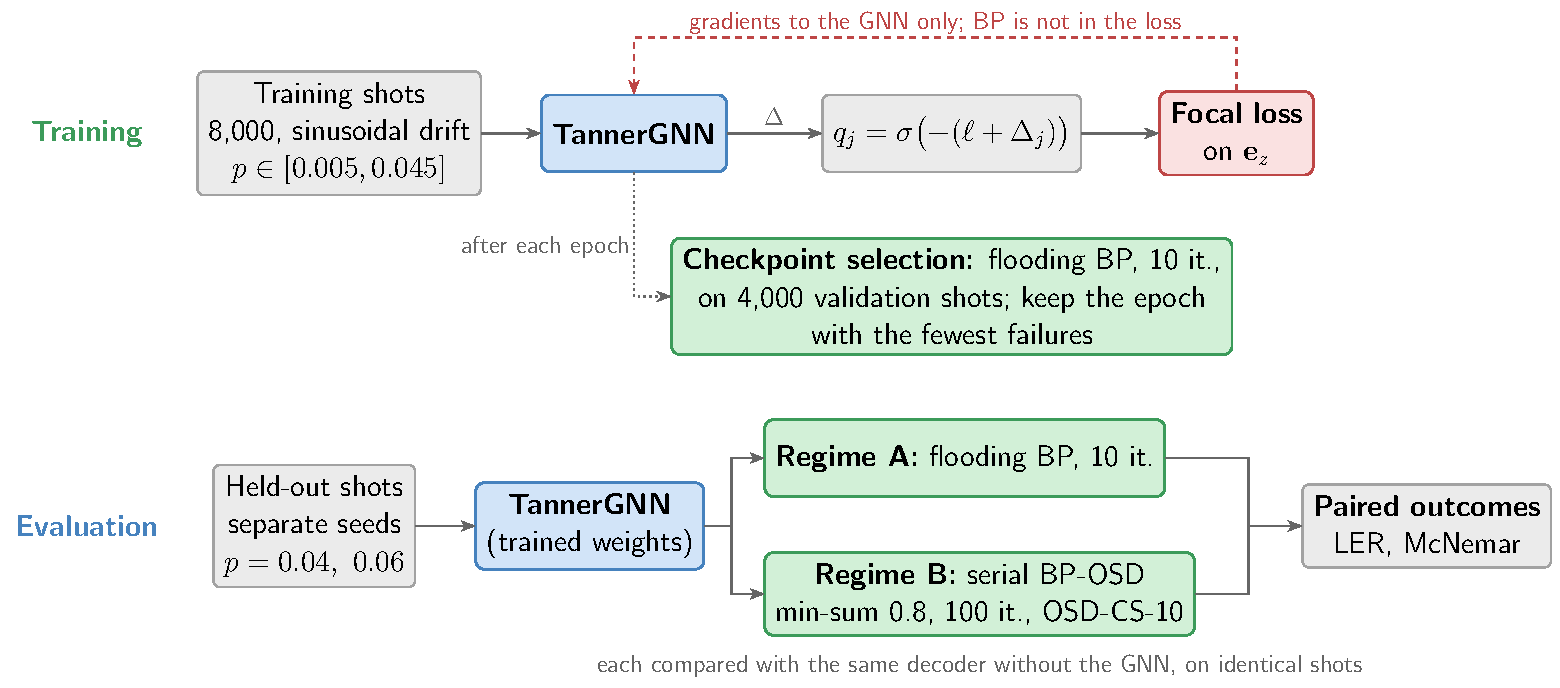
\includegraphics[width=\textwidth]{fig_experimental_pipeline}
\caption{Training and evaluation pipeline of the GNN experiments. The
         GNN is trained with a per-qubit focal loss, without BP in the
         loss; 10-iteration flooding BP selects the checkpoint on
         validation shots. The model is evaluated on separately seeded
         held-out shots in Regime~A (flooding BP) and Regime~B (serial
         BP-OSD); each decoder receives identical syndrome batches to
         enable McNemar paired testing.}
\label{fig:experimental_pipeline}
\end{figure*}

\subsection{Evaluation regimes}\label{sec:regimes}

Two distinct evaluation regimes are used throughout this paper,
and the distinction is central to interpreting the results:

\textbf{Regime A (development baseline):} The GNN is evaluated with
flooding BP, the decoder used to select its checkpoint. This comparison
isolates the gain relative to that decoder.

\textbf{Regime B (stronger reference decoder):} The same learned
correction is evaluated with serial-schedule min-sum BP-OSD
(Table~\ref{tab:hparams}). This tests whether the correction also
improves a stronger classical decoder; BP-OSD serves here as a reference
point, not as the best available decoder (Sec.~\ref{sec:related}). Plain
BP-OSD uses a uniform prior in each component ($p_z$ and $p_x$, or $p$ in
Table~\ref{tab:gnn_null}); the value of a uniform prior does not change its
decisions, which we confirmed on all 20{,}000 test shots at $p=0.04$. With
the GNN, qubit $i$ enters BP-OSD with prior error probability
$\sigma\bigl(-(\ell+\Delta_i)\bigr)$ in both components.
Section~\ref{sec:mismatch} shows that the correction does not help in the
tested regime.

Unless otherwise stated, all experiments use $Z$-biased noise with
$\eta = 20$.

\subsection{Statistical protocol}\label{sec:metrics}

\paragraph{Logical failure.} For each shot let $\hat{e}_z$ and
$\hat{e}_x$ be the decoder's hard decisions and $r_z=e_z\oplus\hat{e}_z$,
$r_x=e_x\oplus\hat{e}_x$ the residual errors. A shot is a logical failure
if (i) the estimate does not reproduce the measured syndrome,
$\Hmat_x\hat{e}_z\neq s_x$ or $\Hmat_z\hat{e}_x\neq s_z$, or (ii) the
syndrome is reproduced but the residual acts nontrivially on the code
space, $\mathbf{L}_x r_z\neq\mathbf{0}$ or $\mathbf{L}_z r_x\neq\mathbf{0}$
over $\F_2$, where the rows of $\mathbf{L}_x$ ($\mathbf{L}_z$) span the
$k=12$ independent logical operators that detect $Z$ ($X$) errors.
Condition (i) is needed because a syndrome-inconsistent residual is not a
logical operator, so its parity against fixed logical representatives is
not meaningful; non-converged BP outputs therefore always count as
failures. The $X$ and $Z$ components are combined by logical OR, so the
reported LER is the probability that at least one of the 12 logical
qubits suffers a logical error of any Pauli type in a shot. At circuit
level the same rule is applied to the detector error model: a shot fails
if the decoded fault set does not reproduce the detection events, or if
it does and predicts the wrong observable flips.

For absolute LER comparisons we treat operating points with fewer than
100 observed logical-error events as preliminary; this is a reporting
heuristic rather than a formal power calculation. Decoder pairs are
evaluated on \emph{identical} syndrome samples, enabling paired
McNemar tests~\cite{McNemar1947} (two-sided, with continuity
correction). We report Wilson score 95\% confidence intervals for LER
estimates.

\paragraph{Comparison families.} Each results table defines one family
of paired tests: the ten GNN-BP vs.\ BP tests of
Table~\ref{tab:gnn_flooding} (two error rates, five seeds), the twenty
GNN+OSD vs.\ BP-OSD tests of Table~\ref{tab:gnn_null} (four error rates,
five seeds), the nine oracle cells of Table~\ref{tab:oracle}, and the GNN
comparisons of the drift experiment (Table~\ref{tab:drift}). Within a
family we control the familywise error rate with Holm's step-down
procedure~\cite{Holm1979} at level 0.05 and say so where adjusted results
are reported; other $p$-values are unadjusted and exploratory. For
emphasized comparisons we report the discordant counts $n_{10}$ and
$n_{01}$, and we never round a $p$-value to zero.

Training, validation and test data are drawn with distinct random
seeds, so no evaluation shot shares a random stream with a training
shot, and learned-decoder results are reported over five training seeds
(initialisation and minibatch order). All training and evaluation used
CPU only; no GPU was available for this work. One training epoch of the
39k-parameter model of Sec.~\ref{sec:gnn_positive} takes about 16\,s.

% ============================================================
%  V. RESULTS
% ============================================================
\section{Results}\label{sec:results}

\subsection{Decoder configuration sensitivity}\label{sec:baseline}

Before presenting the GNN results, we quantify the sensitivity of the
classical baseline to decoder configuration. This sensitivity sets the
scale against which the learned-decoder results must be interpreted.

\begin{table*}[t]
\centering
\caption{Effect of BP-OSD configuration on $\code{288}{12}{18}$,
         $p=0.04$, $\eta=20$, 100{,}000 identical shots, priors $p_z$ and
         $p_x$ of Eq.~\eqref{eq:bias}. 95\% Wilson intervals in brackets.}
\label{tab:smoking_gun}
\begin{tabular}{@{}llllcc@{}}
\toprule
Config & Schedule & Method & Iter & LER & Errors \\
\midrule
Original BP & parallel & prod-sum & 30 & 0.0569 [0.0555,0.0583] & 5{,}689 \\
Reference BP & serial & ms(0.8) & 100 & 0.0017 [0.0015,0.0020] & 174 \\
Original BP-OSD & parallel & prod-sum & 30 & 0.0398 [0.0386,0.0411] & 3{,}983 \\
Ref.\ BP-OSD & serial & ms(0.8) & 100 & 0.00034 [0.00024,0.00048] & 34 \\
\bottomrule
\end{tabular}
\end{table*}

Table~\ref{tab:smoking_gun} illustrates how strongly decoder
configuration changes the finite-length result. The original parallel
product-sum BP-OSD configuration reduces LER from $0.0569$ to $0.0398$
relative to the corresponding plain BP, but remains far worse than the
serial min-sum configurations. The reference serial min-sum BP-OSD
records 34 logical errors in $10^5$ shots, so its value is preliminary
by the criterion of Sec.~\ref{sec:metrics}.

A separate $N=100{,}000$-shot experiment (Fig.~\ref{fig:baseline_decomp})
changes one factor at a time. The flooding comparator is min-sum BP with
scaling factor $0.8$, at most 100 iterations, stopping at the first
iteration whose hard decision satisfies the syndrome, with a parallel
(flooding) schedule; the second decoder is identical except for the
serial schedule; the third adds OSD-CS-10. The LER falls from
$1.28\times10^{-2}$ to $1.45\times10^{-3}$ ($8.8\times$, paired
$n_{10}/n_{01}=1138/3$) and then to $2.7\times10^{-4}$ ($5.4\times$,
$118/0$), about $47\times$ overall.

\begin{figure}[t]
\centering
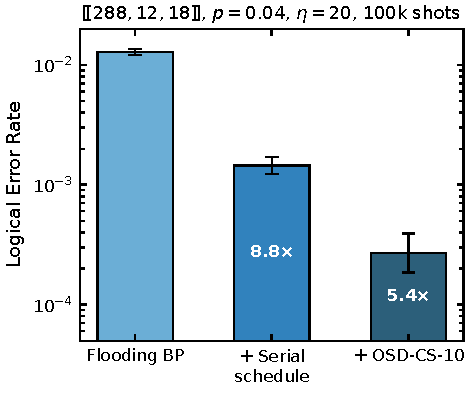
\includegraphics[width=\columnwidth]{fig_F1_baseline_decomp}
\caption{Baseline decomposition on $\code{288}{12}{18}$, $p=0.04$,
         $\eta=20$, 100k identical shots. Min-sum BP (scaling 0.8, at most
         100 iterations) with flooding and then serial schedule, then
         serial BP-OSD-CS-10. Wilson 95\% CI error bars; labels give the
         factor gained at each step.}
\label{fig:baseline_decomp}
\end{figure}

These data do not identify a universally optimal configuration. They do
show that schedule, update rule, iteration budget, and post-processing
can dominate the measured finite-length LER. Learned-decoder comparisons
must therefore specify and control these parameters.

\subsection{Uniform-prior scaling invariance of min-sum BP}\label{sec:invariance}

\begin{proposition}[Uniform positive-scaling invariance]\label{prop:invariance}
Consider separate-CSS min-sum BP with no message clipping or offset. If
all channel LLRs in one CSS component are multiplied by the same factor
$a>0$, then every BP message and posterior LLR is multiplied by $a$ at
every iteration. Consequently, all hard decisions are unchanged.
\end{proposition}

\begin{proof}
At initialization, each variable-to-check message is proportional to the
corresponding channel LLR and therefore scales by $a$. Assume all
variable-to-check messages at iteration $t$ have scaled by $a$. The
syndrome factor $(-1)^{s_j}$ in Eq.~\eqref{eq:ctv} is unchanged, the sign
of every message is unchanged because $a>0$, and
$\min_i a|x_i|=a\min_i|x_i|$. Hence every check-to-variable message also
scales by $a$. Equation~\eqref{eq:vtc} then shows that the next
variable-to-check messages scale by $a$. Induction establishes the claim
for all iterations and for the final posterior LLRs.
\end{proof}

For a uniform channel prior, replacing a common positive LLR $\Lambda$
by another positive value $\Lambda'$ is equivalent to the scaling
$a=\Lambda'/\Lambda$. The proposition explains why changing only the assumed uniform physical
error rate cannot change hard decisions of ideal min-sum BP. Clipping, offsets, damping rules that depend on
magnitude, non-uniform priors, or sum-product updates can break the exact
scaling argument.

We checked the proposition on 2{,}000 shots each. With unclipped
min-sum BP (serial or flooding, 100 iterations), changing the assumed
uniform rate from $p=0.015$ to $p=0.0286$ on $\code{288}{12}{18}$, or from
$p=0.04$ to $p=0.02$ on $\code{72}{12}{6}$, leaves every hard decision
unchanged (2{,}000/2{,}000). Two cases fall outside the proposition, and
the invariance fails there: our PyTorch min-sum implementation clamps
messages to $\pm20$ and changes 18 of 2{,}000 decisions on
$\code{288}{12}{18}$, and sum-product BP changes 25--43 of 2{,}000.

\begin{remark}[What the proposition does and does not imply]
The result applies to the BP pathway when adaptivity enters only by
changing a uniform channel-prior magnitude. It does \emph{not} establish
that a global conditioning scalar is information-theoretically useless
to a GNN: a learned model could combine a global noise estimate with
local syndrome structure and change its nonlinear decision rule. The experiments below test a narrower hypothesis: spatially resolved
per-qubit calibration can change the relative reliabilities seen by the
decoder, whereas a single graph-wide scalar cannot provide that spatial
information.
\end{remark}

\subsection{GNN improvement over flooding BP}\label{sec:gnn_positive}

We evaluated the GNN with flooding BP---the decoder used to select its
checkpoint---on separately seeded held-out syndromes: 4{,}000
validation shots at $p=0.04$ select the checkpoint over 20 epochs, and
test sets of 20{,}000 shots at $p=0.04$ (inside the training range) and
10{,}000 shots at $p=0.06$ (outside it) are each scored once on that
checkpoint. Training is repeated with five seeds.

\begin{table}[t]
\centering
\caption{GNN-BP vs.\ flooding BP on $\code{72}{12}{6}$, $\eta=20$,
         20{,}000 ($p=0.04$) and 10{,}000 ($p=0.06$) held-out test
         syndromes, five training seeds (mean $\pm$ s.d.). $n_{10}$
         ($n_{01}$): shots only BP (only GNN-BP) fails. BP is flooding
         min-sum run for exactly 10 or 100 iterations; the last hard
         decision is used.}
\label{tab:gnn_flooding}
\footnotesize
\setlength{\tabcolsep}{3.5pt}
\begin{tabular}{@{}lcc@{}}
\toprule
 & $p=0.04$ & $p=0.06$ \\
\midrule
BP, 10 iter. & 0.1078 & 0.2867 \\
GNN-BP, 10 iter. & $0.0942\pm0.0006$ & $0.2564\pm0.0019$ \\
\quad relative reduction & $12.5\%\pm0.6\%$ & $10.6\%\pm0.7\%$ \\
\quad $n_{10}$ / $n_{01}$ & 313--370 / 64--95 & 343--394 / 66--80 \\
BP, 100 iter. & 0.0864 & 0.2403 \\
Serial BP-OSD & 0.0707 & 0.2138 \\
\bottomrule
\end{tabular}
\end{table}

Table~\ref{tab:gnn_flooding} gives the primary learned-decoder result.
Over five training seeds, GNN-BP reduces LER relative to flooding BP by
$12.5\%\pm0.6\%$ at $p=0.04$ and by $10.6\%\pm0.7\%$ at $p=0.06$, outside
the training range (McNemar $p<10^{-36}$ for every seed, also after Holm
correction over the ten tests). The gain comes
mostly from convergence: shots on which BP does not reproduce the
syndrome fall from 1{,}740 to 838--975 of 20{,}000. Flooding BP with 100
iterations and serial BP-OSD both remain better than GNN-BP. A gradient
audit on the five checkpoints found non-zero signal through the network
(input-to-readout gradient ratio $0.63$--$2.19$) and non-trivial LLR
corrections (mean $|\Delta_i|=0.54$--$1.01$).

\begin{table}[t]
\centering
\caption{Failures by CSS component on $\code{72}{12}{6}$, $p=0.04$,
         $\eta=20$, 20{,}000 held-out shots (counts). $Z$: $Z$ errors
         decoded on $\Hmat_x$; $X$: $X$ errors decoded on $\Hmat_z$;
         Either: the failure criterion of Sec.~\ref{sec:metrics}. GNN rows
         give the range over five training seeds.}
\label{tab:components}
\footnotesize
\setlength{\tabcolsep}{3pt}
\begin{tabular}{@{}lccc@{}}
\toprule
Decoder & $Z$ & $X$ & Either \\
\midrule
BP, 10 iter. & 2{,}155 & 0 & 2{,}155 \\
GNN-BP, $\Delta$ on both & 1{,}845--1{,}899 & 7--54 & 1{,}874--1{,}906 \\
GNN-BP, $\Delta$ on $Z$ only & 1{,}845--1{,}899 & 0 & 1{,}845--1{,}899 \\
BP, 100 iter. & 1{,}727 & 0 & 1{,}727 \\
Serial BP-OSD & 1{,}414 & 0 & 1{,}414 \\
GNN + BP-OSD & 1{,}439--1{,}451 & 0--1 & 1{,}439--1{,}451 \\
\bottomrule
\end{tabular}
\end{table}

\paragraph{The two CSS components.} Table~\ref{tab:components} separates
the failures at $p=0.04$ by component. All failures of BP, 100-iteration
BP and BP-OSD are in the $Z$ component: at $p_x=0.0019$ none of them
fails on the $X$ component in 20{,}000 shots. The whole GNN gain is
therefore in the $Z$ component. Adding $\Delta$ to the $X$ component as
well, as in Table~\ref{tab:gnn_flooding}, gains nothing there and creates
7--54 $X$-component failures. Adding it to the $Z$ component only removes
them and gives a reduction of $13.3\%\pm0.9\%$ ($10.8\%\pm0.7\%$ at $p=0.06$). This
variant was chosen after seeing the test results, so we keep the
pre-specified setting in Table~\ref{tab:gnn_flooding}. Because BP makes
no $X$-component errors at these operating points, a separately trained
$X$ head would have nothing to correct, and leaving the $X$ prior
unchanged is the appropriate choice. With BP-OSD the $X$ component is
essentially unaffected (at most one extra failure at $p=0.04$), so the
comparisons below do not depend on this choice.

A fixed-dataset capacity test provides an additional diagnostic: a GNN
trained on 1{,}000 fixed syndromes for 50 epochs reduced the failure
count on those same syndromes from 105 to 93 ($11\%$; McNemar
$p=0.0095$, $n_{10}=15$, $n_{01}=3$). This experiment tests the ability of
the architecture and optimizer to fit the supplied examples; it is not a
generalization result. The FiLM and interleaved variants
(Appendix~\ref{app:variants}) are not evaluated in this work.

\subsection{Development/evaluation baseline mismatch}\label{sec:mismatch}

Although the GNN improves flooding BP, the same correction does not
improve the serial min-sum BP-OSD reference configuration. Note that Tables~\ref{tab:gnn_flooding}
and~\ref{tab:gnn_null} report different evaluation regimes
(Regime~A and Regime~B of Sec.~\ref{sec:regimes}) on different
syndrome sets, and their LER values are not directly comparable.

\begin{table}[t]
\centering
\caption{GNN+OSD vs.\ serial BP-OSD on $\code{72}{12}{6}$, $\eta=20$,
         20{,}000 identical shots per $p$, five training seeds (ranges
         over seeds). $n_{10}$ ($n_{01}$): shots only BP-OSD (only
         GNN+OSD) fails. Last two columns: seeds for which GNN+OSD is
         significantly worse (McNemar $p<0.05$), unadjusted and after
         Holm correction over the 20 tests. No seed is significantly
         better.}
\label{tab:gnn_null}
\footnotesize
\setlength{\tabcolsep}{2.5pt}
\resizebox{\columnwidth}{!}{%
\begin{tabular}{@{}lccccc@{}}
\toprule
 & & & & \multicolumn{2}{c}{Seeds worse} \\
$p$ & BP-OSD & GNN+OSD & $n_{10}$ / $n_{01}$ & unadj. & Holm \\
\midrule
0.020 & 0.0093 & 0.0095--0.0102 & 3 / 7--20 & 1/5 & 1/5 \\
0.030 & 0.0297 & 0.0306--0.0317 & 21--28 / 46--64 & 5/5 & 4/5 \\
0.040 & 0.0676 & 0.0688--0.0709 & 52--62 / 84--120 & 4/5 & 2/5 \\
0.050 & 0.1354 & 0.1384--0.1418 & 94--121 / 169--222 & 5/5 & 5/5 \\
\bottomrule
\end{tabular}}
\end{table}

\begin{figure}[t]
\centering
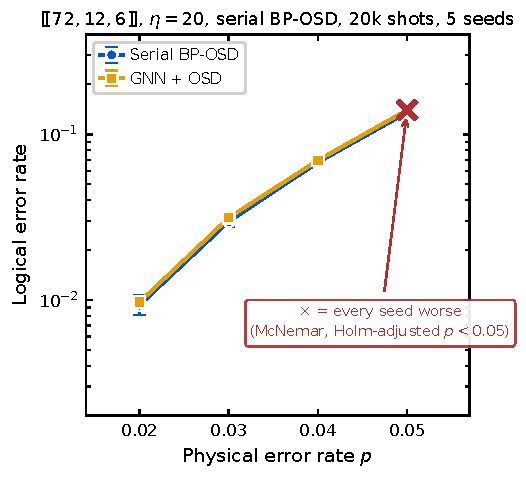
\includegraphics[width=\columnwidth]{fig_F4_phase4_ler}
\caption{GNN+OSD vs.\ serial BP-OSD LER on $\code{72}{12}{6}$,
         $\eta=20$, 20{,}000 shots per point. BP-OSD: Wilson 95\%
         intervals; GNN+OSD: mean over five training seeds, error bars
         give the range over seeds. The red $\times$ marks the operating
         point where every seed is significantly worse after Holm
         correction.}
\label{fig:gnn_null_curve}
\end{figure}

Table~\ref{tab:gnn_null} and Fig.~\ref{fig:gnn_null_curve} show that
the GNN-corrected decoder never improves on serial BP-OSD: no seed is
significantly better at any error rate. Without correction, one seed of
five is significantly worse at $p=0.02$ and 14 of the 15
seed--error-rate pairs are significantly \emph{worse} from $p=0.03$ on;
after Holm correction over the 20 tests, 11 of these 15 remain,
including all five seeds at $p=0.05$. The same checkpoints improve
flooding BP, so these data show that the learned correction does not
transfer unchanged to the stronger decoder.

The GNN checkpoint was selected for 10-iteration flooding BP and is then
inserted ahead of a decoder with a different schedule, iteration budget,
and OSD post-processing.

\begin{table}[t]
\centering
\caption{Paired failure sets on $\code{72}{12}{6}$, $p=0.04$, $\eta=20$,
         20{,}000 identical held-out shots. BP: 10-iteration flooding BP.
         GNN rows give the range over five training seeds. ``Non-conv.'':
         the estimate does not reproduce the syndrome.}
\label{tab:failure_sets}
\footnotesize
\setlength{\tabcolsep}{3pt}
\begin{tabular}{@{}lcc@{}}
\toprule
Decoder & Failures & Non-conv. \\
\midrule
BP, 10 iter. & 2{,}155 & 1{,}740 \\
BP, 100 iter. & 1{,}727 & 700 \\
Serial BP-OSD & 1{,}414 & 0 \\
GNN + BP, 10 iter. & 1{,}874--1{,}906 & 838--975 \\
GNN + BP-OSD & 1{,}439--1{,}451 & 0 \\
\midrule
\multicolumn{3}{@{}l}{\textit{BP vs.\ BP-OSD failure sets}} \\
Both fail & \multicolumn{2}{c}{1{,}319} \\
\makecell[l]{Only BP fails /\\only BP-OSD fails} & \multicolumn{2}{c}{836 / 95} \\
BP fails, given BP-OSD fails & \multicolumn{2}{c}{93\%} \\
BP-OSD fails, given BP fails & \multicolumn{2}{c}{61\%} \\
\makecell[l]{BP-100 failures\\also BP failures} & \multicolumn{2}{c}{1{,}727 / 1{,}727} \\
\midrule
\multicolumn{3}{@{}l}{\textit{What the GNN changes}} \\
Shots GNN fixes for BP & \multicolumn{2}{c}{313--370} \\
\quad of which BP did not converge & \multicolumn{2}{c}{91--93\%} \\
\quad of which BP-OSD also fails & \multicolumn{2}{c}{31--36\%} \\
\makecell[l]{BP-OSD failures also\\GNN+BP failures} & \multicolumn{2}{c}{87--88\%} \\
\makecell[l]{GNN+BP-OSD vs.\ BP-OSD:\\newly failed / rescued} & \multicolumn{2}{c}{237--282 / 206--254} \\
\bottomrule
\end{tabular}
\end{table}

A paired failure-set analysis (Table~\ref{tab:failure_sets}) shows that
the failure sets of BP and BP-OSD overlap strongly but are not nested:
1{,}319 shots fail under both, 836 only under BP and 95 only under
BP-OSD, so 93\% of BP-OSD's failures are BP failures and
61\% of BP's failures are BP-OSD failures. The 100-iteration BP
failures, by contrast, are a strict subset of the 10-iteration ones.
What separates BP from BP-OSD is mainly
convergence: 81\% of BP failures are shots on which BP does not reach a
syndrome-consistent estimate, whereas BP-OSD always returns one. Of the
313--370 shots the GNN fixes for BP, 91--93\% are non-converged BP shots
and only 31--36\% are shots that BP-OSD fails, so the GNN's gains lie
mostly where BP-OSD already succeeds. When the same corrections are
passed to BP-OSD they reshuffle its failures (237--282 newly failed vs.\
206--254 rescued shots), almost entirely among shots on which BP itself
fails. The same pattern holds at $p=0.06$, where 96\% of BP-OSD failures
are BP failures (and 71\% the other way). Training directly against
the target decoder, or against a differentiable surrogate of its
post-processing stage, remains the appropriate test of whether learned
augmentation can improve BP-OSD.

\begin{table}[t]
\centering
\caption{Classes of the BP failures on $\code{72}{12}{6}$ at $p=0.04$
         (10-iteration flooding BP, traced for 100 iterations) and of the
         shots the GNN repairs (range over five seeds). ``Met'': the hard
         decision reproduces the syndrome. A symmetric
         configuration is a $Z$ error covering three qubits of a
         weight-six $Z$ stabilizer.}
\label{tab:mechanism}
\footnotesize
\setlength{\tabcolsep}{3pt}
\begin{tabular}{@{}lcc@{}}
\toprule
Class & BP failures & GNN repairs \\
\midrule
Wrong class (syndrome met) & 415 & 22--32 \\
Transient (met before it.~10) & 78 & 5--11 \\
Slow (met by it.~100) & 1{,}030 & 249--265 \\
Oscillating (never met) & 631 & 37--78 \\
Stuck (never met) & 1 & 0 \\
\midrule
Total & 2{,}155 & 313--370 \\
\quad symmetric configuration & 606 & 89--137 \\
\bottomrule
\end{tabular}
\end{table}

\paragraph{Which failures the GNN repairs.} To see what kind of failure
the correction repairs, we traced flooding BP for 100 iterations on the
$p=0.04$ test set (Table~\ref{tab:mechanism}). Of the 2{,}155 BP
failures, 415 reach a syndrome-consistent estimate in the wrong logical
class. The other 1{,}740 do not reproduce the syndrome after 10
iterations: 78 had reproduced it earlier and moved away, 1{,}030
reproduce it later, 631 never reproduce it and keep changing their hard
decision, and one is stuck. Stopping each shot at its first
syndrome-consistent iteration would change the BP failure count only from
2{,}155 to 2{,}146, so the fixed iteration budget is not a handicap of the
baseline. The shots the GNN repairs are mostly slow ones (249--265 of
313--370), followed by oscillating (37--78) and wrongly converged
(22--32) shots: the correction mainly speeds up convergence.

A recurring structure among the failures is a symmetric stabilizer
configuration~\cite{Raveendran2021Trapping}: the $Z$ error covers exactly
three qubits of a weight-six $Z$ stabilizer $g$, so that $e_z$ and
$e_z\oplus g$ have the same weight and syndrome and are logically
equivalent. Such configurations occur in 3.5\% of the test shots but in
28\% of BP failures; BP fails on 87\% of the shots that contain one and on
8\% of the others. Error weight does not explain this. On all
57 weight-three errors of this kind, BP, 100-iteration BP and GNN-BP with
every seed fail, while BP-OSD fails on none (24 of 24 and none at
$p=0.06$); on the 4{,}466 weight-three errors without such a
configuration BP fails on 2.4\%. The GNN lowers BP's failure rate on
symmetric configurations from 87\% to 67--74\%, all of it on configurations of
weight four and more; on the weight-three ones it never helps, as expected
from its loss (Sec.~\ref{sec:training}). OSD resolves the tie by
construction, which is one reason why many BP failures are not BP-OSD
failures.

\subsection{Per-qubit calibration gap}\label{sec:oraclegap}

Under spatially non-uniform per-qubit noise, each data qubit has rate
$p_i=p\,e^{\sigma z_i-\sigma^2/2}$ with $z_i\sim\mathcal N(0,1)$ drawn
fresh every shot (capped at 0.5), so the mean rate is $p$ for every
$\sigma$; the $Z$ and $X$ rates of qubit $i$ are $p_i\eta/(\eta+1)$ and
$p_i/(\eta+1)$. A decoder knowing the true per-qubit rates (serial min-sum
BP-OSD-CS-10 with the true $p_i$ as priors) substantially outperforms a
decoder using the uniform mean prior $p$.

\begin{figure}[t]
\centering
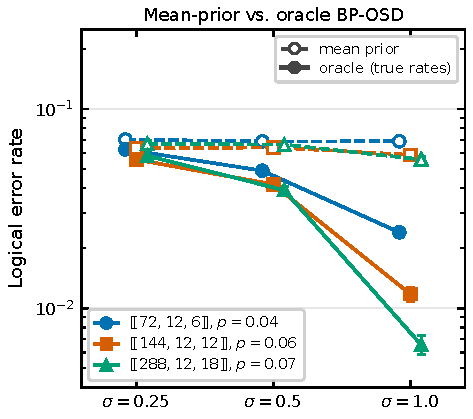
\includegraphics[width=\columnwidth]{fig_F2_oracle_gap}
\caption{Mean-prior and oracle serial BP-OSD LER with Wilson 95\%
         intervals, 50{,}000 identical shots per point. Each code is
         shown at its own operating point ($p=0.04$, $0.06$, $0.07$);
         because code size and operating point change together, the
         figure does not show a distance trend.}
\label{fig:oracle_gap}
\end{figure}

\begin{table*}[t]
\centering
\caption{Oracle gap: LER of mean-prior and per-qubit (oracle) serial
         BP-OSD with Wilson 95\% intervals, 50{,}000 identical shots per
         row; the three codes are at different operating points.
         Reduction: $1-\mathrm{LER}_\mathrm{oracle}/\mathrm{LER}_\mathrm{mean}$.
         $n_{10}$ ($n_{01}$): shots only the mean-prior decoder (only the
         oracle) fails. All nine McNemar $p<10^{-22}$, also after Holm
         correction.}
\label{tab:oracle}
\small
\setlength{\tabcolsep}{4pt}
\begin{tabular}{@{}lcccccc@{}}
\toprule
Code ($d$) & $p$ & $\sigma$ & Mean prior & Oracle & Reduction & $n_{10}$ / $n_{01}$ \\
\midrule
$\code{72}{12}{6}$ (6) & 0.04 & 0.25 & 0.0702 [0.0680,0.0724] & 0.0626 [0.0605,0.0647] & 11\% & 681 / 301 \\
 &  & 0.5 & 0.0686 [0.0665,0.0709] & 0.0489 [0.0471,0.0509] & 29\% & 1{,}340 / 355 \\
 &  & 1.0 & 0.0688 [0.0666,0.0710] & 0.0240 [0.0227,0.0254] & 65\% & 2{,}435 / 198 \\
$\code{144}{12}{12}$ (12) & 0.06 & 0.25 & 0.0633 [0.0612,0.0655] & 0.0557 [0.0537,0.0577] & 12\% & 924 / 543 \\
 &  & 0.5 & 0.0641 [0.0619,0.0662] & 0.0418 [0.0401,0.0436] & 35\% & 1{,}485 / 371 \\
 &  & 1.0 & 0.0587 [0.0567,0.0608] & 0.0118 [0.0109,0.0128] & 80\% & 2{,}441 / 94 \\
$\code{288}{12}{18}$ (18) & 0.07 & 0.25 & 0.0668 [0.0646,0.0690] & 0.0582 [0.0562,0.0603] & 13\% & 1{,}089 / 662 \\
 &  & 0.5 & 0.0661 [0.0640,0.0684] & 0.0391 [0.0374,0.0408] & 41\% & 1{,}804 / 450 \\
 &  & 1.0 & 0.0557 [0.0537,0.0578] & 0.0065 [0.0059,0.0073] & 88\% & 2{,}525 / 66 \\
\bottomrule
\end{tabular}
\end{table*}

Table~\ref{tab:oracle} and Fig.~\ref{fig:oracle_gap} show a clear
increase with noise contrast $\sigma$ for each tested code. The reported
percentage reduction is also larger for the larger-code rows, reaching
$88\%$ on $\code{288}{12}{18}$ at $\sigma=1.0$; however, the physical
error rate is changed across codes ($p=0.04$, $0.06$, and $0.07$).
Consequently, these data do not isolate code distance as the cause of
the cross-code trend. At a common operating point ($p=0.04$, $\sigma=1$)
the reductions are 65\%, 85\% and 88\% for the three codes, but the
two larger codes record only 278 and 17 mean-prior failures there, so
this controlled comparison is preliminary.

This experiment isolates the value of synthetic per-qubit rate side
information; it does not require machine learning. We use the true-rate
decoder as an \emph{oracle reference}, not as a formal upper bound on all
possible decoders. The comparison quantifies how much the tested BP-OSD
implementation can benefit when the realized per-qubit rates are
revealed. When the field is redrawn independently for every shot, these
rates are not identifiable from that shot's syndrome: averaged over the
field, the errors of each CSS component are independent across qubits
with the uniform rates $p_z$ and $p_x$, exactly as under uniform noise, so
a component's syndrome carries no information about the realized field.
(The field does correlate the $X$ and $Z$ errors of a qubit, which a joint
decoder could exploit; ours decode the components separately.) A
syndrome-only decoder could still outperform mean-prior BP-OSD by being a
better decoder for i.i.d.\ noise, but such a gain would not come from
estimating the $p_i$.

\subsection{Drift adaptation}\label{sec:drift}

We test whether per-qubit rate estimates help BP-OSD when the rates
drift. On $\code{72}{12}{6}$ with mean rate $p=0.04$ and $\eta=20$, each
data qubit $i$ has a log-rate offset $x_i(t)$ that follows a discrete
Ornstein--Uhlenbeck (AR(1)) process, independently across qubits,
\begin{equation}
x_i(t+1)=\rho\,x_i(t)+v\,\xi_i(t),\qquad \rho=\sqrt{1-v^2/\sigma^2},
\label{eq:ou}
\end{equation}
with $\xi_i(t)\sim\mathcal N(0,1)$, $x_i(0)\sim\mathcal N(0,\sigma^2)$ and
$\sigma=1$, so the stationary spread of the log-rates is $\sigma$ for every
volatility $v$. The volatility is the per-shot standard deviation of the
log-rate innovation: $v=0$ is a static field, and $v=0.1$, $0.35$ and $0.5$
give correlation times $-1/\ln\rho$ of about 200, 15 and 7 shots. The rate
of qubit $i$ at shot $t$ is $p_i(t)=\min\bigl(0.5,\,p\,e^{x_i(t)-\sigma^2/2}\bigr)$,
whose stationary mean is $p$, and each shot draws independent $Z$ and $X$
flips with probabilities $p_i\eta/(\eta+1)$ and $p_i/(\eta+1)$.

All decoders are serial min-sum BP-OSD (Table~\ref{tab:hparams}) with
per-qubit priors $\hat p_i\eta/(\eta+1)$ and $\hat p_i/(\eta+1)$; they
differ only in the rate estimate $\hat p_i(t)$. The \emph{oracle} uses the
true $p_i(t)$. \emph{Stale} uses $p_i(0)$, a perfect calibration taken at
the start of the stream and never updated. \emph{Mean} uses the uniform
rate $p$. \emph{Empir} counts the $Z$ flips $n_i$ in its own decoded
estimates over the previous $W=32$ shots and shrinks the frequency toward
$p$ with $K=16$ pseudo-shots,
$\hat p_i=\frac{\eta+1}{\eta}\,\bigl(n_i+Kp\eta/(\eta+1)\bigr)/(W+K)$.
\emph{GNN} is a \textsc{TannerGNN} rate estimator with the architecture of
Table~\ref{tab:hparams} that maps the violated-check frequencies of the
previous $W$ syndromes to an estimate $\hat x_i(t)$ and sets
$\hat p_i=\min\bigl(0.5,\,p\,e^{\hat x_i-\sigma^2/2}\bigr)$; it sees
syndromes only, never decoder outputs or true rates. It is trained by
mean-squared error on 20{,}000 windows drawn at the four volatilities,
with five training seeds; for each seed the epoch with the lowest
validation error out of 30 is kept. Every decoder sees the current
syndrome. Each volatility is evaluated on 20 independent streams of
2{,}532 shots, whose first 32 shots are warm-up and not scored, giving
50{,}000 scored shots. Shots in one stream share a rate field, so pooled
McNemar tests overstate the evidence; we therefore compare decoders by a
sign test over the 20 streams, with Holm correction over the eight GNN
comparisons.

\begin{table*}[t]
\centering
\caption{Drift experiment on $\code{72}{12}{6}$, $p=0.04$, $\eta=20$,
         $\sigma=1$, $W=32$: LER of serial BP-OSD with different per-qubit
         rate estimates, 50{,}000 scored shots (20 streams) per
         volatility $v$. GNN: range over five training seeds. Last two
         columns: streams on which the seed-averaged GNN has fewer / more
         failures than stale calibration and than the empirical
         estimator.}
\label{tab:drift}
\begin{tabular}{@{}lccccccc@{}}
\toprule
$v$ & Oracle & Stale & Mean & Empir & GNN & vs.\ stale & vs.\ empir \\
\midrule
0.00 & 0.0210 & 0.0210 & 0.0645 & 0.0333 & 0.0428--0.0433 & 0/20 & 0/20 \\
0.10 & 0.0223 & 0.0747 & 0.0655 & 0.0358 & 0.0474--0.0477 & 20/0 & 0/20 \\
0.35 & 0.0232 & 0.0821 & 0.0682 & 0.0541 & 0.0602--0.0607 & 20/0 & 0/20 \\
0.50 & 0.0243 & 0.0819 & 0.0678 & 0.0601 & 0.0648--0.0651 & 20/0 & 0/20 \\
\bottomrule
\end{tabular}
\end{table*}

\begin{figure}[t]
\centering
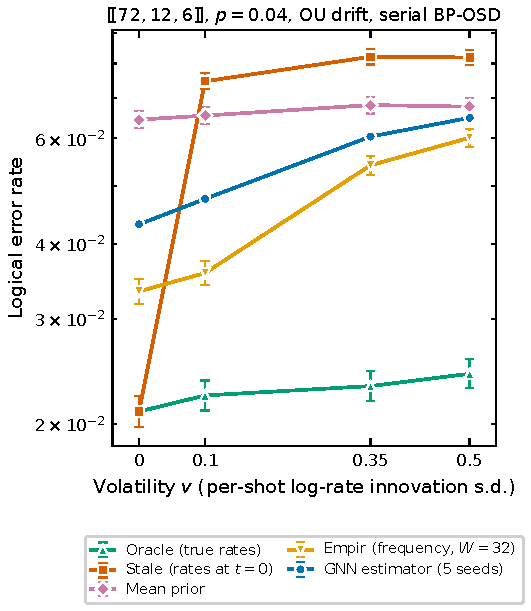
\includegraphics[width=\columnwidth]{fig_F3_drift_adaptation}
\caption{LER of serial BP-OSD under per-qubit OU drift against the
         volatility $v$ on $\code{72}{12}{6}$, $p=0.04$, $\sigma=1$, for
         five rate estimates. Wilson 95\% intervals; for the GNN, the mean
         over five training seeds with the range over seeds.}
\label{fig:drift_curve}
\end{figure}

Table~\ref{tab:drift} and Fig.~\ref{fig:drift_curve} show three things.
First, a per-qubit calibration is valuable only while it is current.
Without drift the stale calibration is the oracle (LER 0.0210, against
0.0645 for the mean prior), but at $v=0.1$, where the rates decorrelate over
about 200 shots, it is already worse than the mean prior (0.0747 vs.\
0.0655). Second, tracking the rates recovers much of the gap: the
non-learned frequency estimator reaches 0.0333 without drift and 0.0358 at
$v=0.1$, and its advantage shrinks as the correlation time approaches the
window length (0.0601 vs.\ 0.0678 for the mean prior at $v=0.5$). Third,
the GNN estimator beats stale calibration at every nonzero volatility and
the mean prior at every volatility (on all 20 streams up to $v=0.35$ and
on 17 of 20 at $v=0.5$), but it is worse than the frequency estimator
on all 20 streams at every volatility; all eight GNN comparisons
remain significant after Holm correction. The five training seeds give
nearly identical results. Under independent per-qubit drift, counting each
qubit's decoded errors therefore captures more of the available signal
than the learned syndrome-based estimator; whether spatially correlated
drift would change this is an open question.

\subsection{Circuit-level evaluation}\label{sec:circuit}

\paragraph{Circuit and noise model.} We simulate a $Z$-basis memory
experiment on $\code{72}{12}{6}$ with 6 rounds of syndrome extraction
(72 data qubits, 36 $X$-check and 36 $Z$-check ancillas). Data qubits are
prepared in $\ket{0}$; each round measures all $X$-checks and then all
$Z$-checks with dedicated ancillas, using CNOT layers from a greedy
conflict-free schedule; the data qubits are finally measured in the $Z$
basis. Detectors are (i) the 36 $Z$-checks of round 1, which are
deterministic for the prepared state, (ii) the XOR of consecutive
measurements of every check in rounds 2--6, and (iii) the XOR of the last
$Z$-check outcome with the parity of the measured data qubits in its
support, giving 432 detectors and 12 logical observables. The noise,
summarized in Table~\ref{tab:circuitnoise}, is a custom biased Pauli
model, not standard circuit-level depolarizing noise: every one- and
two-qubit gate is followed by an independent single-qubit channel on each
qubit it acts on, with mutually exclusive $X$ and $Z$ faults and no $Y$
fault, so a two-qubit gate has no correlated two-qubit faults. Under
spatially non-uniform noise each qubit $q$ (data and ancilla) has rate
$p_q=p\,e^{\sigma z_q-\sigma^2/2}$, $z_q\sim\mathcal N(0,1)$, $\sigma=1$,
on all of its fault locations, so the mean rate is $p$ as in
Sec.~\ref{sec:oraclegap}.

\begin{table}[t]
\centering
\caption{Circuit noise for a qubit $q$ with rate $p_q$ ($p_q=p$ under
         uniform noise), $\eta=20$. Each line acts independently on
         every qubit concerned.}
\label{tab:circuitnoise}
\footnotesize
\setlength{\tabcolsep}{3pt}
\begin{tabular}{@{}ll@{}}
\toprule
Location & Fault \\
\midrule
After reset to $\ket{0}$ & $X$, prob.\ $p_q$ \\
\makecell[l]{After $H$ or CNOT\\(each qubit)} & \makecell[l]{$X$, prob.\ $p_q/(\eta+1)$, or\\$Z$, prob.\ $p_q\eta/(\eta+1)$} \\
\makecell[l]{Idle qubit,\\each time step} & as after a gate \\
Before $Z$ measurement & outcome flip, prob.\ $p_q$ \\
\bottomrule
\end{tabular}
\end{table}

\paragraph{Decoders.} Stim~\cite{Gidney2021Stim} converts each noisy
circuit into a detector error model (DEM) with 4{,}068 fault mechanisms on
432 detectors. Each mechanism collects the circuit faults that flip the
same detectors and observables, and its prior is their combined
probability; the exclusive $X$ and $Z$ outcomes of a channel are treated
as independent faults (Stim's \texttt{approximate\_disjoint\_errors}). The
mean-prior decoder uses the DEM of the circuit with every qubit at rate
$p$, and the oracle uses the DEM of the circuit with each qubit at its true
rate $p_q$; the two DEMs have the same mechanisms and differ only in their
priors. Both are decoded with serial min-sum BP-OSD (scaling 0.8, 100
iterations, OSD-CS order 10), as in Table~\ref{tab:hparams}. We draw 20
rate profiles at $p\le0.003$ and 40 at $p=0.01$, with 500 shots per
profile. Failures follow Sec.~\ref{sec:metrics}.

\begin{table}[t]
\centering
\caption{Circuit-level oracle gap on $\code{72}{12}{6}$ (6 rounds,
         $\eta=20$, $\sigma=1$). LER in percent with Wilson 95\%
         intervals. $n_{10}$ ($n_{01}$): shots only the mean-prior decoder
         (only the oracle) fails.}
\label{tab:circuit}
\footnotesize
\setlength{\tabcolsep}{2.5pt}
\resizebox{\columnwidth}{!}{%
\begin{tabular}{@{}lcccccc@{}}
\toprule
$p$ & Shots & Mean prior & Oracle & $n_{10}$ & $n_{01}$ & $p_\mathrm{McN}$ \\
\midrule
0.001 & 10{,}000 & 0 [0,0.04] & 0 [0,0.04] & 0 & 0 & --- \\
0.003 & 10{,}000 & 0 [0,0.04] & 0 [0,0.04] & 0 & 0 & --- \\
0.01 & 20{,}000 & 1.35 [1.19,1.51] & 0.60 [0.50,0.72] & 177 & 28 & $5\!\times\!10^{-25}$ \\
\bottomrule
\end{tabular}}
\end{table}

\begin{figure}[t]
\centering
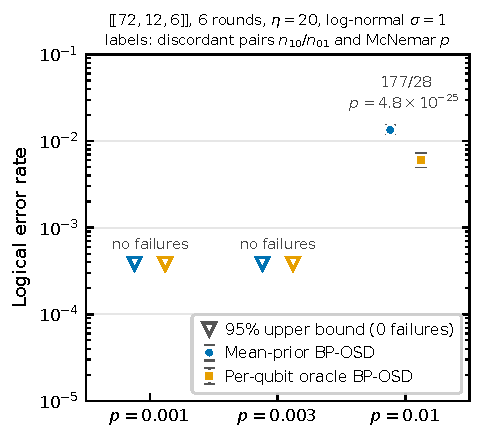
\includegraphics[width=\columnwidth]{fig_F6_circuit_oracle}
\caption{Circuit-level oracle gap on $\code{72}{12}{6}$, 6 rounds,
         $\eta=20$, $\sigma=1$. Points: LER with 95\% Wilson intervals;
         open triangles: 95\% upper bound when no failures were
         observed. Labels: discordant pairs and McNemar $p$.}
\label{fig:circuit_null}
\end{figure}

Knowing the per-qubit rates also helps at circuit level
(Table~\ref{tab:circuit}, Fig.~\ref{fig:circuit_null}). At $p=0.01$ the
oracle reduces the logical error rate from $1.35\%$ to $0.60\%$ ($55\%$;
McNemar $p=4.8\times10^{-25}$), and it is better on 38 of 40 independent
rate profiles (sign test $p=1.5\times10^{-9}$), so the result is not
driven by a few extreme profiles. At $p=0.001$ and $p=0.003$ neither
decoder fails in $10^4$ shots, so these operating points cannot resolve a
gap. The circuit-level gap is somewhat smaller than the code-capacity gap
on the same code ($65\%$ at $\sigma=1$, Table~\ref{tab:oracle}), at a
different operating point, but it does not vanish.

% ============================================================
%  VI. DISCUSSION
% ============================================================
\section{Discussion}\label{sec:discussion}

\subsection{The GNN's role and its limits}

\textsc{TannerGNN} reduces the LER of the flooding BP decoder used to
select its checkpoint by $12.5\%\pm0.6\%$ over five training seeds, and
gradient diagnostics show that the network produces non-trivial
corrections. The gain comes mainly from helping BP converge on shots where
it converges slowly, and 100-iteration BP and serial BP-OSD remain
stronger than the corrected decoder.

The Regime-B result is also informative: the learned correction does
not transfer automatically to serial BP-OSD. This is consistent with the
mismatch between the development and evaluation decoders: most BP-OSD
failures are also BP failures, and the GNN's repairs fall mostly on shots
BP-OSD already decodes (Table~\ref{tab:failure_sets}). The symmetric
stabilizer configurations of Sec.~\ref{sec:mismatch} show the reverse
case: failures that BP-OSD avoids by construction and that a bitwise loss
cannot teach the GNN to repair. Training against BP-OSD directly is
complicated by the non-differentiable OSD stage; differentiable
surrogates, distillation, training on the residual failures of the target
decoder, or a degeneracy-aware loss~\cite{Liu2019Neural} are possible
alternatives.

\subsection{Benchmark design implications}

The baseline experiments identify two reporting requirements for learned
QLDPC decoders. First, BP-OSD schedule, update rule, iteration count, and
OSD configuration must be stated explicitly because they can change LER
by more than two orders of magnitude on the same code. Table~\ref{tab:hparams}
records these settings for the present study.

Second, the decoder used for model selection and the evaluation decoder
must be distinguished. An LLR correction selected for flooding BP need not
remain beneficial
when the schedule, iteration count, and OSD stage are changed. Comparisons
across such decoder configurations should identify the mismatch rather
than treating all BP-based baselines as equivalent.

\subsection{Comparison with prior work}\label{sec:priorwork}

Astra~\cite{Maan2025MLBP} uses a learned Tanner-graph message-passing
decoder and reports BB-code performance competitive with, and in several
settings better than, BP-OSD under code-capacity depolarizing noise. This
places our $12.5\%$ flooding-BP gain in context: improvement over plain BP
is not, by itself, the main novelty. Our contribution is instead the
controlled comparison showing how that gain changes when the baseline
and side information are strengthened.

Gong et al.~\cite{Gong2024GNN} interleave differentiable BP stages with
GNN corrections on the same sparse graph and show error-floor
improvements over several post-processing approaches. Our interleaved
variant (Appendix~\ref{app:variants}) follows the same broad design
principle, but its decoding performance is not evaluated here, so we do
not claim a competitive result for that architecture.

Recent circuit-level work on BB codes also reports neural decoders that
can outperform BP-OSD on the $\code{72}{12}{6}$ code while retaining a
runtime advantage, although scaling to $\code{144}{12}{12}$ remains more
challenging~\cite{Blue2026MLBB}. This comparison reinforces the need to evaluate learned decoders against
a fully specified strong non-learned baseline, not only against
flooding BP.

Stein et al.~\cite{Stein2026FiLM} condition a neural QEC decoder on
spatially resolved hardware calibration data using FiLM and evaluate on
IBM repetition-code experiments. Their conditioning signal is per-qubit
and calibration-derived, unlike the single global rate $p$ fed to our
FiLM variant (Appendix~\ref{app:variants}). This distinction is consistent with the oracle experiments
of Sec.~\ref{sec:oraclegap}, which motivate spatial rather than purely
global conditioning.
\subsection{Towards spatially-resolved conditioning}\label{sec:srcf}

The oracle-gap experiment (Sec.~\ref{sec:oraclegap}) shows that
per-qubit rate side information can materially improve the tested
BP-OSD decoder. Because operating point and code size co-vary, the
current data do not establish how this value scales with distance.
Proposition~\ref{prop:invariance} also shows that a uniform rescaling
of the min-sum BP prior cannot reproduce the effect of spatially varying
reliabilities. These results motivate testing spatially resolved FiLM
(SRCF), in which per-qubit parameters $(\gamma_i, \beta_i)$ are
conditioned on persistent hardware calibration data rather than on a
single graph-wide scalar. Soft syndrome information~\cite{Raveendran2023Soft}
is another form of side information that iterative decoders can use. Such
a decoder should be compared with the
non-learned frequency estimator of Sec.~\ref{sec:drift} and evaluated
in a circuit-level setting where the calibration signal remains
identifiable. Neither condition has been established in the present
experiments.

\subsection{Limitations}\label{sec:limitations}

\begin{enumerate}[leftmargin=*,topsep=3pt,itemsep=2pt,
                  label=(\roman*)]
\item The evaluated GNN was trained with a per-qubit loss and
      selected for 10-iteration flooding BP; no model was trained or
      selected for serial BP-OSD, our reference decoder. Whether GNN
      augmentation of serial BP-OSD yields gains is untested.
\item GNN checkpoints exist only for $\code{72}{12}{6}$; the
      larger codes were not trained due to CPU-only compute
      constraints. The null result in Regime B should not be
      extrapolated to the larger codes.
\item The interleaved and FiLM architectures
      (Appendix~\ref{app:variants}) are described but their decoding
      performance is not evaluated.
\item The correction is trained on $Z$ errors and, in the headline
      setting, also added to the $X$ component, where it only adds
      failures (Table~\ref{tab:components}); the $Z$-only setting was
      chosen after seeing the test results.
\item The training loss is not degeneracy-aware (Sec.~\ref{sec:training}).
\item Code-capacity noise omits measurement errors, leakage,
      and correlated faults present in real circuits, and the circuit
      model uses independent single-qubit channels rather than
      correlated two-qubit faults.
\item The drift experiment is synthetic: the rates of different qubits
      drift independently, with correlation times of 7 to 200 shots.
\end{enumerate}

% ============================================================
%  VII. CONCLUSION
% ============================================================
\section{Conclusion}\label{sec:conclusion}

On $\code{72}{12}{6}$, a Tanner-graph GNN whose checkpoint is selected
with 10-iteration flooding BP reduces the held-out LER of that decoder by
$12.5\%\pm0.6\%$ at $p=0.04$ over five training seeds, all of it in the
$Z$ component. The same correction never improves serial min-sum BP-OSD
and is often significantly worse; it mostly repairs shots on which BP
converges slowly and which BP-OSD already decodes. Weight-three errors
that cover half of a stabilizer defeat BP with or without the GNN but
never BP-OSD, and the bitwise training loss cannot teach the network to
break that tie. The demonstrated gain is therefore specific to the
flooding-BP baseline.

BP schedule, update rule, iteration budget and OSD configuration change
the finite-length LER by orders of magnitude, so they belong to the
decoder specification. A uniform rescaling of the channel LLRs cannot
change min-sum decisions, whereas the true per-qubit rates reduce
BP-OSD's LER by up to 88\% under synthetic heterogeneous noise and by 55\%
under circuit-level noise. Under per-qubit drift a stale calibration quickly loses its
value, and a simple frequency estimator tracks the rates better than a
learned one. A natural next test is a
decoder conditioned on persistent spatial calibration data, trained with a
degeneracy-aware loss, and compared with fully specified BP-OSD and the
frequency estimator.
\section*{Acknowledgments}

The authors thank the STAR Lab program at the University of Arizona
for facilitating this research and providing computational resources.

\section*{Data and code availability}

{\raggedright All code, data, trained checkpoints and per-shot outcomes
behind every table and figure are available at
\url{https://github.com/kondshk/adaptive_gnn} (tag \texttt{paper-v5}).
The script \texttt{make\_tables.py} rebuilds every results table from the
stored outcomes, and \texttt{requirements-lock.txt} lists the exact
package versions. Code-capacity data are sampled directly with NumPy;
circuit-level data are generated with Stim~\cite{Gidney2021Stim}.\par}

\bibliographystyle{quantum}
\bibliography{references}

\appendix

\section{Unevaluated variants}\label{app:variants}

The code base contains two further variants of the model. Neither is
evaluated in this paper, and no result in the main text depends on them.

\paragraph{FiLM conditioning.} Feature-wise Linear Modulation
(FiLM)~\cite{Perez2018FiLM} conditions each GNN layer on an external
context. A small generator network maps a global noise level to per-layer
affine parameters $(\gamma^{(\ell)}, \beta^{(\ell)})$, which modulate the
aggregated messages as $\gamma^{(\ell)} \odot \bvec{m}^{(\ell)} +
\beta^{(\ell)}$ (Fig.~\ref{fig:tannergnn_arch}). In the implementation the
generator receives the physical error rate $p$ of the shot, i.e.\ the true
global rate rather than an estimate from the syndrome. This input is one
scalar shared by the whole graph and contains no per-qubit reliability
information. Proposition~\ref{prop:invariance} shows that uniformly
rescaling the channel prior cannot change the hard decisions of unclipped
min-sum BP; it does not imply that a GNN cannot use a global scalar as
context.

\paragraph{Neural BP.} Differentiable BP generalises
Eqs.~\eqref{eq:vtc}--\eqref{eq:ctv} with learnable per-iteration weights on
the channel LLR, the variable-to-check messages and the check-to-variable
messages, $w^{(t)} = \mathrm{softplus}(w_\mathrm{raw}^{(t)})/\ln 2$.
Dividing by $\ln 2$ makes $w_\mathrm{raw}=0$ give $w=1$ exactly, so at
initialisation the unrolled network is standard min-sum BP with scaling
factor 0.8.

\paragraph{Interleaved pipeline.} Algorithm~\ref{alg:interleaved} and
Fig.~\ref{fig:interleaved_pipeline} give the interleaved pipeline. The GNN
intervenes twice: before BP to correct channel priors, and after $T_1$
iterations using the intermediate posterior information. Qubits with
$p_i^\mathrm{mid} \approx 0.5$ have low posterior confidence and can
receive a second learned correction. Unlike the model of
Sec.~\ref{sec:training}, both correction stages are trained jointly
through the differentiable BP unroll, so the loss is computed on BP's
output marginals. The FiLM and interleaved variants are trained on data
regenerated each epoch with $p\sim\mathrm{Uniform}[0.01,0.10]$, with the
focal loss on both components and a syndrome-consistency term, the binary
cross-entropy between the measured syndrome and
$\tfrac12\bigl(1-\prod_{j\in\mathcal N(c)}(1-2q_j)\bigr)$ for each check
$c$, with weight $0.1$.

\begin{algorithm}[t]
\DontPrintSemicolon
\SetAlgoLined
\caption{Interleaved GNN-BP Decoding}\label{alg:interleaved}
\KwIn{$\synd$, channel LLR $\llr$, global noise level $p$}
\KwOut{Error estimate $\ehat$}
$(\gamma,\beta) \leftarrow \mathrm{FiLMGen}(p)$\tcp*{Conditioning}
$\Delta^{(1)} \leftarrow \textsc{TannerGNN}(\llr, \synd, \gamma, \beta)$\;
$\llr' \leftarrow \llr + \Delta^{(1)}$\tcp*{Prior correction}
$\llr_\mathrm{mid} \leftarrow \mathrm{NeuralBP}(\llr', \Hmat, T_1)$\;
$p_i^\mathrm{mid} \leftarrow \sigma(-\llr_{\mathrm{mid},i})\;\forall i$\;
$\Delta^{(2)} \leftarrow \textsc{TannerGNN}(\llr_\mathrm{mid}, p^\mathrm{mid}, \synd, \gamma, \beta)$\;
$\llr'' \leftarrow \llr_\mathrm{mid} + \Delta^{(2)}$\tcp*{Mid correction}
$\llr_\mathrm{final} \leftarrow \mathrm{NeuralBP}(\llr'', \Hmat, T_2)$\;
$\hat{e}_i \leftarrow \mathbbm{1}[\llr_{\mathrm{final},i} < 0]\;\forall i$\;
\Return{$\ehat$}
\end{algorithm}

\begin{figure*}[t]
\centering
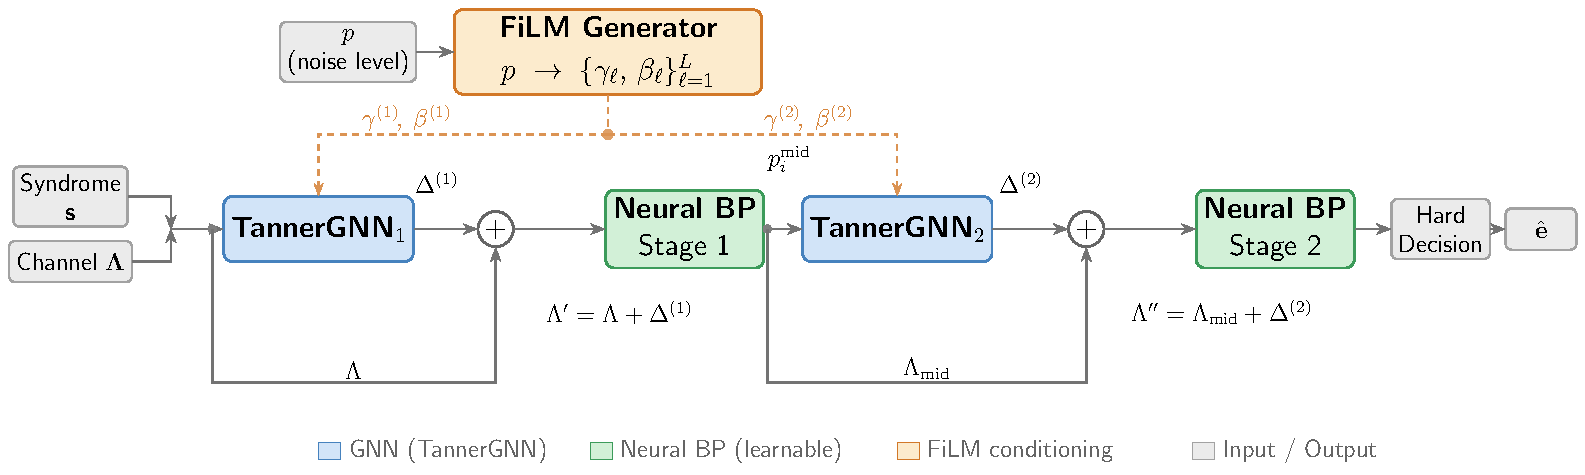
\includegraphics[width=\textwidth]{fig_interleaved_pipeline}
\caption{Interleaved GNN-BP pipeline. The GNN applies two successive
         LLR corrections: one before BP initialisation and one after
         $T_1$ iterations, using the mid-decoding posterior as an
         additional input. Both stages are trained end-to-end through
         the BP unroll. This variant is not evaluated in this paper.}
\label{fig:interleaved_pipeline}
\end{figure*}

\end{document}
